
\documentclass{article}
\usepackage[landscape]{geometry}
\usepackage{url}
\usepackage{multicol}
\usepackage{amsmath}
\usepackage{esint}
\usepackage{amsfonts}
\usepackage{tikz}
\usetikzlibrary{decorations.pathmorphing}
\usepackage{amsmath,amssymb}
\usetikzlibrary{shadows}
\usepackage{colortbl}
\usepackage{xcolor}
\usepackage{mathtools}
\usepackage{amsmath,amssymb}
\usepackage{enumitem}
\usepackage{setspace}
\usepackage{hyperref}
\makeatletter

\newcommand*\bigcdot{\mathpalette\bigcdot@{.5}}
\newcommand*\bigcdot@[2]{\mathbin{\vcenter{\hbox{\scalebox{#2}{$\m@th#1\bullet$}}}}}
\makeatother

\title{CSA Cheat Sheet}
\usepackage[brazilian]{babel}
\usepackage[utf8]{inputenc}

\advance\topmargin-.8in
\advance\textheight3in
\advance\textwidth3in
\advance\oddsidemargin-1.5in
\advance\evensidemargin-1.5in
\parindent0pt
\parskip2pt
\newcommand{\hr}{\centerline{\rule{3.5in}{1pt}}}
%\colorbox[HTML]{e4e4e4}{\makebox[\textwidth-2\fboxsep][l]{texto}
\begin{document}

\begin{multicols*}{3}

\definecolor{NYUpurple}{RGB}{79, 15, 134}
\tikzstyle{mybox} = [draw=NYUpurple, fill=white, very thick,
    rectangle, rounded corners, inner sep=10pt, inner ysep=10pt]
\tikzstyle{fancytitle} =[fill=NYUpurple, text=white, font=\bfseries]


%------------ Mixing ---------------
\begin{tikzpicture}
\node [mybox] (box){%
    \begin{minipage}{0.3\textwidth}
    \begin{multicols}{2}
        \begin{itemize}
        \item $n_x$: number of x
        \item $T_x$: time of x
        \item $P_x$: percentage or power of x
        \item $i$: instructions
    \end{itemize}
    
    \end{multicols}

    \end{minipage}
};
%------------ Mixing Header ---------------------
\node[fancytitle, right=10pt] at (box.north west) {Notation};
\end{tikzpicture}


%------------ Mixing ---------------
\begin{tikzpicture}
\node [mybox] (box){%
    \begin{minipage}{0.3\textwidth}
    Speed Up Ratio: $\frac{T_{Prev}}{T_{Current}} = \frac{\text{Throughput current}}{\text{Throughput previous}}$
    
    SPECratio = $\frac{T_{ref}}{T_{current}}$, where reference times means baseline time in an \textbf{benchmark}

    The execution time imporved = $\frac{T_{Prev}-T_{Current}}{T_{Prev}}$

    Throughput: $\frac{n_{data}}{T_{exec}}$, maxIPS:$\frac{n_{instruction}}{T_{exec}}$

    program maxIPS = $\sum_{i \in prog} maxIPS_i \times P_i$ 

    Performance Per Wat = $\frac{maxIPS}{Power}$, Not Throughtput

    MIPS: Millions of Instructions Per Second
    
    \end{minipage}
};
%------------ Mixing Header ---------------------
\node[fancytitle, right=10pt] at (box.north west) {Basic conecpt};
\end{tikzpicture}

%------------ Heating ---------------
\begin{tikzpicture}
\node [mybox] (box){%
    \begin{minipage}{0.3\textwidth}
    % content here
    CPI: Average cycles per instruction, \textbf{not reverse}
    $$
    \mathrm{CPI}=\frac{n_{cycles}}{n_{instruct}} \leftrightarrow  n_{cycles} = CPI\times n_{instruct}
    $$ 
    $$T_{execution} = CPI\times n_{instruct} \times T_{clock} = \frac{CPI\times n_{instruct}}{\text{CLK Rate}}$$
    
    Clock Rate vs Clock Time are Reciprocal
    $$
    \text{CLK Rate} = \frac{n_{cycle}}{T_{execution}} , \text{CLK Time} = \frac{T_{execution}}{n_{cycle}}
    $$
    Clock Rate vs Clock Time's Unit
    \begin{multicols}{2}
        \begin{itemize}
            \renewcommand{\itemsep}{0pt} % 项目之间的间距
            \renewcommand{\parsep}{0pt}  % 段落之间的间距
            \item 1 kHz = \(10^3\) Hz 
            \item 1 MHz = \(10^6\) Hz
            \item 1 GHz = \(10^9\) Hz 
            \item 1 s = \(10^3 \, \text{ms}\)
            \item 1 s = \(10^6 \, \mu s\)
            \item 1 s = \(10^9 \, ns\)
        \end{itemize}
    \end{multicols}
    
    \end{minipage}
};
%------------ Heating Header ---------------------
\node[fancytitle, right=10pt] at (box.north west) {Clock Rate/Time/CPI};
\end{tikzpicture}



%------------ Inner Product Spaces ---------------
\begin{tikzpicture}
\node [mybox] (box){%
    \begin{minipage}{0.3\textwidth}
    \textbf{1}: Run a benchmark on different HW, different in CPI/$n_{instruct}$/CLK Rate
    
    \textbf{2}: Bearkdown a program by to FP,INT,L/S,Branch, change attributes accordingly     \textbf{Notice}: 


    \begin{itemize}
        \item Use table to record data of HW or instructions
        \item Use the right formula $\frac{CPI\times n_{instruct}}{\text{CLK Rate}}$
        \item Different in Speed Up Ratio and Time saved
        \item Some speed up ratio may not achieved IRL
    \end{itemize}

    Eg: 1-1, 1-6, 1-10
    \end{minipage}
};
%------------ Inner Product Space Header ---------------------
\node[fancytitle, right=10pt] at (box.north west) {Problem Template for Clock Cycle};
\end{tikzpicture}

%------------ Gram-Schmidt Content ---------------
\begin{tikzpicture}
\node [mybox] (box){%
    \begin{minipage}{0.3\textwidth}
    $
    S = \frac{1}{(1 - P) + \frac{P}{N}}
    $, P is Parallel ratio and N is P speed up

    In some probles, we have Parallel overhead

    Eg: 1-2, 1-5, 1-11
    \end{minipage}
};
%------------ Gram-Schmidt Header ---------------------
\node[fancytitle, right=10pt] at (box.north west) {Amdahl's law};
\end{tikzpicture}
%------------ Variation of Parameters Content ---------------------
\begin{tikzpicture}
\node [mybox] (box){%
    \begin{minipage}{0.3\textwidth}
    Power = $C \times V^2 \times f$ W 
    
    Energy = $C \times V^2$ J
    \end{minipage}
};
%------------ Variation of Parameters Header ---------------------
\node[fancytitle, right=10pt] at (box.north west) {Power and Energy of HW};
\end{tikzpicture}

\begin{tikzpicture}
\node [mybox] (box){%
\begin{minipage}{0.3\textwidth}

Shut down some machine/Change chip attribute/Change running state(aka. power comsumption) and Calculate power/energy change, note:
\begin{itemize}
    \item Shut down P \% machine $\rightarrow $ save P \% energy
    \item Note power/energy change are different, where \textbf{energy has no relation with frenquent}
\end{itemize}

Eg: 1-7

\end{minipage}
};
%------------ Variation of Parameters Header ---------------------
\node[fancytitle, right=10pt] at (box.north west) {Power and Energy of Problem Template};
\end{tikzpicture}



%------------ ODE Content ---------------
\begin{tikzpicture}
\node [mybox] (box){%
    \begin{minipage}{0.3\textwidth}
    MTTF: Mean Time To Failure, $MTTF=\frac{1}{FIT}$
    
    FIT:Failure In Time, $FIT_{system}=\frac{FIT_{single}}{P_{system fail} }$ TODO 

    Eg: 1-4
    \end{minipage}
};
%------------ ODE Header ---------------------
\node[fancytitle, right=10pt] at (box.north west) {QoS};
\end{tikzpicture}

%------------ Series Solution Content ---------------
\begin{tikzpicture}
\node [mybox] (box){%
    \begin{minipage}{0.3\textwidth}
    \textbf{Moore's Law}: number of transistors on a microchip doubles approximately every two years, exponential.

    \textbf{Power Wall} refers to a limitation in computer architecture related to power consumption and heat dissipation, causing Moore's Law no longer work.

    \textbf{Multicore architects} doing with the extra transistors now to increase performance Eg:1-8
    \end{minipage}
};
%------------ Series Solution Header ---------------------
\node[fancytitle, right=10pt] at (box.north west) {Moore's Law and the Power Wall};
\end{tikzpicture}


%------------ Systems of ODE Content ---------------
\begin{tikzpicture}
\node [mybox] (box){%
    \begin{minipage}{0.3\textwidth}
    a/b/c:value in register, A/B/C:address in register
    \begin{multicols}{2}
    \begin{itemize}
    \item \texttt{c=a-b} : sub x,a,b
    \item \texttt{c=a+1} : addi x,a,1
    \item \texttt{A=a} : sw a, 0(A)
    \item \texttt{b=B} : lw b, 0(B)
    \item \texttt{a=a<<2} or \texttt{a=a*4}: slli a,a,2
    \end{itemize}
    \end{multicols}
    Eg: 2-1
    \end{minipage}
};
%------------ Systems of ODE Header ---------------------
\node[fancytitle, right=10pt] at (box.north west) {RISCV Translation Basic};
\end{tikzpicture}

\begin{tikzpicture}
\node [mybox] (box){%
    \begin{minipage}{0.3\textwidth}
    \href{https://github.com/scatyf3}{@scayf3} , CC-BY-4.0
    \end{minipage}
};
\end{tikzpicture}

%------------ Systems of ODE Content ---------------
\begin{tikzpicture}
\node [mybox] (box){%
    \begin{minipage}{0.3\textwidth}
    Indexing: $\texttt{slli} \rightarrow  \text{add start and offset} \rightarrow lw/sw$

    \begin{align*}
    \underbrace{ x_1 = \underbrace{ A[\underbrace{i}_{\texttt{slli i, i,2}}]}_{\texttt{add i, A, i}}}_{\texttt{lw x1, 0(i)}} \quad\quad&
    \underbrace{\underbrace{A[\underbrace{i}_{\texttt{slli i, i,2}}]}_{\texttt{add i, A, i}} =  x_1}_{\texttt{sw x1, 0(i)}}
    \end{align*}

    Loop: couter init $\rightarrow$ LOOP tag/branch $\rightarrow$ counter step $\rightarrow$ loop body $\rightarrow$ jump back/end tag
    \begin{tabular}{|l|l|}
        \hline
        \texttt{int i = 10;} & \texttt{addi x1, 10, x0} \\
        \hline
        \texttt{while (i >= 0)} & \texttt{LOOP:beq x1, x0, DONE} \\
        \hline
        \texttt{i--} & \texttt{addi x1, x1, -1} \\
        \hline
        (Loop Body) & (Loop Body) \\
        \hline
        \texttt{\}} (end of loop) & \texttt{jal x0, LOOP} \\
        \hline
        (end of loop) & \texttt{DONE} \\
        \hline
    \end{tabular}
    
    Eg: 2-1, 2-5, 2-6
    \end{minipage}
};
%------------ Systems of ODE Header ---------------------
\node[fancytitle, right=10pt] at (box.north west) {RISCV Translation Advance};
\end{tikzpicture}


%------------ Systems of ODE Content ---------------
\begin{tikzpicture}
\node [mybox] (box){%
    \begin{minipage}{0.3\textwidth}
    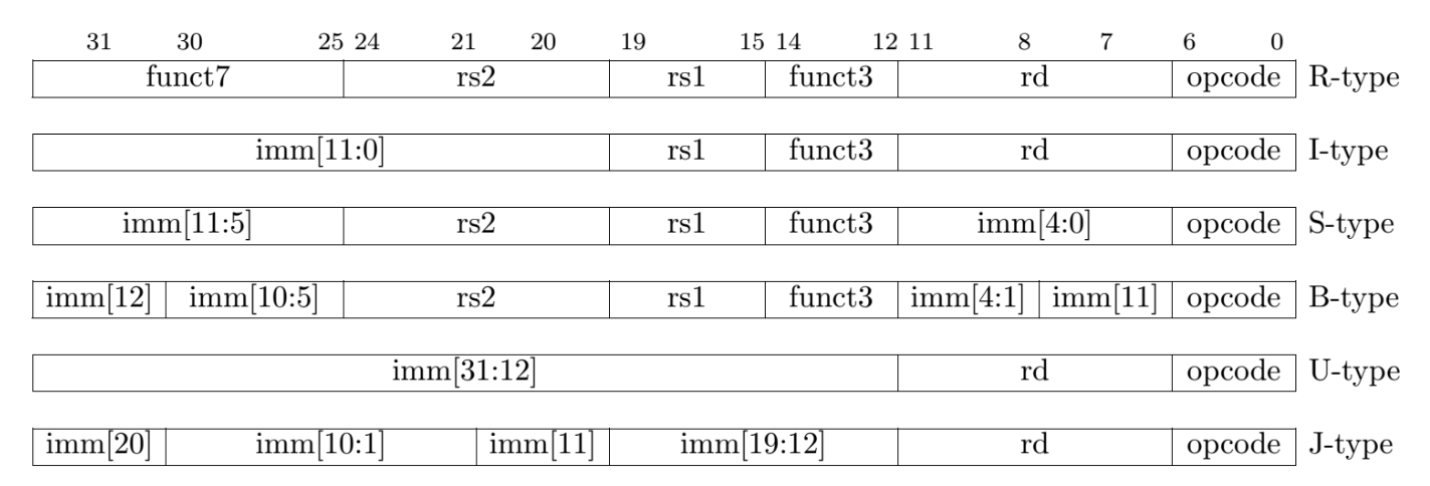
\includegraphics[width=1\linewidth]{image.png}
    
    Eg: 2-2
    \end{minipage}
};
%------------ Systems of ODE Header ---------------------
\node[fancytitle, right=10pt] at (box.north west) {RISCV format};
\end{tikzpicture}

%------------ Systems of ODE Content ---------------
\begin{tikzpicture}
\node [mybox] (box){%
    \begin{minipage}{0.3\textwidth}
    Given instruction, check it's binary code, Eg: 2-3

    Since imm field is limit, calculate some upper/lower bound, Eg: 2-5

    Imm
    \begin{itemize}
        \item I: 12bits, \texttt{addi}'s imm value's bound, unsign/signed
        \item S: 12 bits, \texttt{sw}'s offset's bound, raw address
        \item B: 13 bits, raw address
        \item U: large imm, 20bits
        \item J: range to jump, 21bits
    \end{itemize}

    B and J imm layout: both of them has no 0 bits, that's because the target address is always 2-byte aligned(32bits), the last byte is meaningless. 
    
   
    \end{minipage}
};
%------------ Systems of ODE Header ---------------------
\node[fancytitle, right=10pt] at (box.north west) {RISCV format Problem Template};
\end{tikzpicture}

%------------ Exponentiation Content ---------------
\begin{tikzpicture}
\node [mybox] (box){%
    \begin{minipage}{0.3\textwidth}
    Shift 4n in binary(default) = shift n in hex
    
    Shift meaning: $\underset{\text{shift}}{s}\overset{\text{ left or right}}{r}  \underset{\text{logic or arithmetic}}{l} \overset{\text{immediate} }{i}$

    Logical: and/andi, or/ori, xor/xori ; Note: andi = select bits, ori $\approx$ add 2 binary , xori 0xFF = not

    Eg: 2-2, 2-4
    \end{minipage}
};

%------------ Spring-Mass Header ---------------------
\node[fancytitle, right=10pt] at (box.north west) {Jump and Branch};
\end{tikzpicture}
\
%------------ Laplace Transforms Content ---------------
\begin{tikzpicture}
\node [mybox] (box){%
    \begin{minipage}{0.3\textwidth}
    Jump: jal(address=imm), jalr(address=reg+imm)

    Branch: \texttt{b<condition>}, if condition==true jump
    
    subtype: beq, bne, blt, bge(signed), xxx u(unsigned)

    \textbf{ORDER} \texttt{blt, rs1, rs2, Label}: if $rs1 < rs2$ jump 
    

    Eg: 2-6
    \end{minipage}
};


%------------ Spring-Mass Header ---------------------
\node[fancytitle, right=10pt] at (box.north west) {Bit op};
\end{tikzpicture}
\
%------------ Laplace Transforms Content ---------------
\begin{tikzpicture}
\node [mybox] (box){%
    \begin{minipage}{0.3\textwidth}
    $$
    n_{i} = n_{loop} \times n_{\text{i in loop}} + n_{\text{i out loop}}+ \underbrace{1}_{\text{jump out of loop}}
    $$

    Eg: 2-6, 2-7
    \end{minipage}
};
%------------ Laplace Transforms Header ---------------------
\node[fancytitle, right=10pt] at (box.north west) {Loop Instruction Counts};
\end{tikzpicture}
%------------ Gaussian Integral Content ---------------------
\begin{tikzpicture}
\node [mybox] (box){%
    \begin{minipage}{0.3\textwidth}
	$$
    \begin{array}{cccccc}

    Memory & 0 & 1 & 2 & 3 &\text{0x12345678}\\
    \hline
    \text{big endian} & 12 & 34 & 56 & 78 & \text{MSB in low address} \\
    \text{little endian} & 78 & 56 & 34 & 12 & \text{LSB in low address}
    \end{array}
    $$

    Note: both memory and data are in hex, Eg: 2-8
\end{minipage}
};
%------------ Gaussian Integral Header ---------------------
\node[fancytitle, right=10pt] at (box.north west) {Big/Little Endian};
\end{tikzpicture}

%------------ Gaussian Integral Content ---------------------
\begin{tikzpicture}
\node [mybox] (box){%
    \begin{minipage}{0.3\textwidth}
    Load Upper Immediate \texttt{lui} or Add Upper Immediate to PC \texttt{auipc}, Eg: 2-9(load 64 bits)

    To load 0xABCD1234(32bits) to x10: 
    \begin{verbatim}
    lui x10, 0xABCD1 // [31:12]
    addi x10, x10, 0x234 // [11:0]
    \end{verbatim}
    
\end{minipage}
};
%------------ Gaussian Integral Header ---------------------
\node[fancytitle, right=10pt] at (box.north west) {U instruction};
\end{tikzpicture}

\begin{tikzpicture}
\node [mybox] (box){%
    \begin{minipage}{0.3\textwidth}
    

    \begin{tikzpicture}[
     auto,                % some style definitions of the elements follow
     node distance = 0cm, % used in this picture
     bin/.style    = {rectangle, fill=white, text=black},
     dec/.style    = {draw=none, text=black},
    circ/.style    = {circle, top color=white, bottom color=blue!50,
    draw=blue, very thin, minimum size=5.25cm, drop shadow={opacity=0.5}}
  ]
  % draw a grid in the background
  \draw[step=1,gray,thin] (-4,-4) grid (4,4);
  \node[circ] (center) at (0,0)  {};
  \node[font=\sffamily]   (4bit)   at (0,.5) {4 bit};

  % Simply hand calculated angles for the positions of the bit values
  %varound the circle

  \foreach \angle / \bits in {%
      0/0000, 22.5/0001, 45/0010, 67.5/0011, 90/0100, 112.5/0101,
    135/0110, 157.5/0111, 180/1000, 202.5/1001, 225/1010, 247.5/1011,
    270/1100, 292.5/1101, 315/1110, 337.5/1111}
    \draw (\angle:3.25cm) node [bin, font=\ttfamily] {\bits};

  \draw[fill=red, opacity=.25]
    (-4,-4) -- (-4cm,.8cm) -- (4cm,-0.7cm) -- (4cm,-4cm) -- cycle;

  % Simply hand calculated angles for the positions of
  % the decimal values around the circle

  \foreach \angle / \dez in {%
    0/0, 22.5/1, 45/2, 67.5/3, 90/4, 112.5/5, 135/6, 157.5/7, 180/-8,
    202.5/-7, 225/-6, 247.5/-5, 270/-4, 292.5/-3, 315/-2, 337.5/-1}
    \draw (\angle:2.25cm) node [dec, font=\sffamily] {\dez};

  \foreach \angle / \bits in {%
      0/0000, 22.5/0001, 45/0010, 67.5/0011, 90/0100, 112.5/0101,
    135/0110, 157.5/0111, 180/1000, 202.5/1001, 225/1010, 247.5/1011,
    270/1100, 292.5/1101, 315/1110, 337.5/1111}
    \draw (\angle:3.25cm) node [bin, fill=none, font=\ttfamily] {\bits};
\end{tikzpicture}

Since register are 64 bits, the range of int/uint is

int: $[2^{-31},2^{31}-1]$, uint: $[0,2^{32}-1]$, Eg: 2-10

\end{minipage}
};
%------------ Gaussian Integral Header ---------------------
\node[fancytitle, right=10pt] at (box.north west) {Two's complement and valid range};
\end{tikzpicture}





\end{multicols*}
\end{document}


Contact GitHub API Training Shop Blog About
© 2016 GitHub, Inc. Terms Privacy Security Status Help